%%%%%%%%%%%%%%%%%%%%%%%%%%%%%%%%%%%%%%%%
%% MCM/ICM LaTeX Template %%
%% 2022 MCM/ICM           %%
%%%%%%%%%%%%%%%%%%%%%%%%%%%%%%%%%%%%%%%%
\documentclass[12pt]{article}
\usepackage{geometry}
\geometry{left=1in,right=0.75in,top=1in,bottom=1in}

%%%%%%%%%%%%%%%%%%%%%%%%%%%%%%%%%%%%%%%%
% Replace ABCDEF in the next line with your chosen problem
% and replace 1111111 with your Team Control Number
\newcommand{\Problem}{A}
\newcommand{\Team}{2200655}
%%%%%%%%%%%%%%%%%%%%%%%%%%%%%%%%%%%%%%%%

\usepackage{newtxtext}
\usepackage{amsmath,amssymb,amsthm}
\usepackage{newtxmath} % must come after amsXXX

\usepackage{graphicx}
\usepackage{xcolor}
\usepackage{fancyhdr}
%%%%%%%%%%%%%%%%%%%%%%%%%%%%%%%%%%%%%%%%
\usepackage{lipsum}
\usepackage{tabularx}
\usepackage{epstopdf}
\usepackage{mathrsfs}
\usepackage{longtable}
\usepackage{cite}
\usepackage{makecell}
\usepackage{diagbox}
\lhead{Team \Team}
\rhead{}
\cfoot{}

\newtheorem{theorem}{Theorem}
\newtheorem{corollary}[theorem]{Corollary}
\newtheorem{lemma}[theorem]{Lemma}
\newtheorem{definition}{Definition}

%%%%%%%%%%%%%%%%%%%%%%%%%%%%%%%%
\begin{document}
\graphicspath{{./figure/}}  % Place your graphic files in the same directory as your main document
\DeclareGraphicsExtensions{.pdf, .jpg, .tif, .png}
\thispagestyle{empty}
\vspace*{-16ex}
\centerline{\begin{tabular}{*3{c}}
        \parbox[t]{0.3\linewidth}{\begin{center}\textbf{Problem Chosen}\\ \Large \textcolor{red}{\Problem}\end{center}}
         & \parbox[t]{0.3\linewidth}{\begin{center}\textbf{2022\\ MCM/ICM\\ Summary Sheet}\end{center}}
         & \parbox[t]{0.3\linewidth}{\begin{center}\textbf{Team Control Number}\\ \Large \textcolor{red}{\Team}\end{center}} \\
        \hline
    \end{tabular}}
%%%%%%%%%%% Begin Summary %%%%%%%%%%%
% Enter your summary here replacing the (red) text
% Replace the text from here ...
\begin{center}
    \textbf{Summary}
\end{center}

An energy storage system allows you to capture electricity, store it as another form of energy (battery, thermal, mechanical),
and then have it available to use when needed. The purpose of these storage units is to store energy produced during sunny daylight hours for use when the solar
panels do not produce enough energy for the demand (night or cloud-covered), or for storage and transfer of excess energy. Of the solar-powered homes that use an energy storage system,
most use some sort of battery. Some homeowners have only one large battery, while others may use a “bank of batteries” (two or more batteries connected). Energy storage can be expensive
and so homeowners should choose a system that is appropriate for their situation

Our model is aimed to find the best solution for such a system, we use the method of Linear Programming to find the best solution that
cost the least while having enough capacity and power to support all the appliance at home.

Therefor, we should find the requirements for the house. The first requirement that we need to know
is the capacity needed for the appliance to run long enough, to do so, we find some data form the
EIA's RECS report in 2015 To
know how many electrical appliances are there in a family of three people, then we divide the energy need by
3 and times it with the population in a 1600 feet home, which attained by dividing the area with the
Per capita housing size in the United States. With the same method that we find the requirement
of maximum power.

And then we looked at two different scenarios, the first is to use replaceable  batteries only,
they will have no such thing as Instantaneous Power Rating, which makes the system more vulnerable
to any sudden increasement  of the power that is usually caused by so high power appliances like
the hairdryer. So it must have a higher power, the requirement for power became $\sum_{i=1}^2PiXi\geq M+K$, which is later proved very unhelpful in cutting the budget

The second scenario is that we use a mixture of replaceable batteries and lithium Batteries, which
turned the requirement for maximum power to be $\sum_{i=3}^5I_iX_i\geq M+K$. In fact, we found that the lithium Batteries are so superior that we should actually use them only.

After finding the best solution for this home, we generalized the model to make it now capable of finding the solution for different homes with different area and with different optional batteries.
We still looked at two different scenarios, and we take the area as a variable, so does the number of types of the two kinds of batteries so that we can discuss them separately.

The following work is about a different kind of battery: the cement battery, we discussed the proper way to add it into our model and made a list of the information that we need to do so.
\newline \begin{center}
    \textbf{keywords:}\Large Linear Programming, Energy Storage System, Lithium Batteries Cement battery, Replaceable Batteries, Instantaneous Power Rating.

\end{center}
\textbf{Follow us @COMAPMath on Twitter or COMAPCHINAOFFICIAL on Weibo for the \newline
    most up to date contest information.}


% to here
%%%%%%%%%%% End Summary %%%%%%%%%%%

%%%%%%%%%%%%%%%%%%%%%%%%%%%%%%
\clearpage
\pagestyle{fancy}
% Uncomment the next line to generate a Table of Contents
%\tableofcontents 
\newpage
\setcounter{page}{1}
\rhead{Page \thepage\ }
%%%%%%%%%%%%%%%%%%%%%%%%%%%%%%
\title{Storing the Sun:a Model for Off-grid Power System Design}
\Large
\maketitle
\tableofcontents   % 若不想要目录, 注释掉该句
\newpage
%%%%%%%%%%%%%%%%%%%%%%%%%%%%%%%%%%%%%%%%%%%%%%%%%%
\section{Introduction}
\subsection{Background}

There are many types of bicycle road races including a criterium, a team time trial, and an
individual time trial. A rider’s chance of success can vary for these contests depending on the
type of event, the course, and the rider’s abilities. In an individual time trial, each individual
cyclist is expected to ride a fixed course alone, and the winner is the rider who does so in the
least amount of time.

An individual rider can produce different levels of power for different lengths of time, and the
amount of power and how long a given amount of power a rider can produce varies greatly
between riders. A rider’s power curve indicates how long a rider can produce a given amount of
power. In other words, for a particular length of time the power curve provides the maximum
power a rider can maintain for that given time. Generally, the more power a rider produces, the
less time the rider can maintain that power before having to reduce the amount of power and
recover. A rider may choose to briefly exceed the limits on their power curve, but the rider then
requires extra time at a lower power level to recover. Moreover, a rider’s power output in the
past matters, and riders are increasingly fatigued as a race progresses.

Riders are always looking to minimize the time required to cover a given distance. Given a
particular rider’s capability according to that rider’s power curve, how should that rider apply
power while traversing a given time trial course? Additionally, many types of riders may
participate in an individual time trial, such as a time trial specialist, a climber, a sprinter, a
rouleur, or a puncheur, and each type of rider has a distinct power curve.

Our team aims to establish a model that can give the optimal plan for any particular rider, which tells them exactly when to accelerate,
and when to slow down so that they can make the best of themselves.
\subsection{Restatement of the Problem}
\subsubsection{Requirement 1}
First we shall define a few "volunteers" to test our model, we need them to be various, we shall choose two different types of rider, time trial
specialists and climbers, and we will define a male and a female for each of the two types of riders.
\subsubsection{Requirement 2}
We are now required to identify the parameters that we need to\
use to measure "similarity" in music
characteristics and the proper way to combine them with different scalars. Then with the method,
and the data in the 3 files "full\_music\_data"
"data\_by\_artist", "data\_by\_year",
we were able to find out whether  artists
within genre  are more similar  than artists between genres

\subsubsection{Requirement 3}
It might not be so wise to try to analyze the influence and the development of music directly or only from the data for different musicians, we need a way to simplify our question.
We think it's' the best to categorize the musicians, it can not only help us simplify our work, but also  improves the generality of our method.
When we listen to some music, it seems that we can always classify them into a certain genre, yet there are always controversy, so first, we need a better way to identify the genres, thus we can analyze
the similarity and relationship between different genres.
\subsubsection{Requirement 4}
Now that we had finished the construction of the directed network
of musical influence, we should now use similarity to indicate whether the similarity data can support
that the identified influencers in fact influence the respective
artists as reported in the data\_influence data set. And if there are some characteristics that tend to be high between a pair of influencer and follower, we will be
considered more "contagious".
\subsection{Requirement 5}
In the history of genres, there are always changes and development, sometime the change can happen in a sudden, some characteristics will change in a short period,
we will analyze the changes
of different characteristics to see if there are some that happened in a sudden. And those songs don't' write themselves,
there have to be artists represent revolutionaries, we will analyze them, we will find those who has great influence in a revolution.
\subsubsection{Requireemt 6}
However, as Roman was not built in one day, the changes of a genre is not always abrupt, it is more often than not that changes will not change basic characteristics of
a genre, we will find the history of a music genre, and those who are behind them, namely, those "dynamic influencers", we will develop a new parameter
that reveal the dynamic influencers.
\subsubsection{Requirement 7}
Music is a universal language, a perfect tool to express our emotion and our feeling and express our demands, most of us absolutely love music. We are compelled by it. We are provoked by it.
We are moved by it. We are inspired by it. We feel connected to it. It reflects something profound about who we are and our experience of the world. And the most popular
genre of the Expanding this further, strong support existed in early ethnomusicological literature for the idea that music can tell us many things about a particular culture through its instruments,
instrument makers, and its performance structures that encompass the interaction between performers, audience and/orcomposers (Lomax, 1976; Merriam, 1964; Spearritt, 1980). Lomax`s (1976) work is still
significant in this area, as it explored the specific way that culture was reflected in music practice and it highlighted a correlation between social structure and
song structure. Lomax (1976) believed that a culture`s song performance style “has a special cultural and social role to play among human communication systems” (p. 12).
Even earlier, Lomax (1968) had written that “a culture`s favoured song style reflects and reinforces the kind of behaviour essential to its main subsistence efforts and
to its central and controlling social institutions” (p. 133). Further, Held`s (1984) work with
the Kaluli people in the highlands of Papua New Guinea demonstrated a similar relationship between social structures and musical experience as discovered by Lomax (1976).
In a word, music has a deep connection with culture and society, we will try to find a way to show the influence, find what features in our graph indicate changes of the
society.
\section{Assumptions and Justification}

To simplify the problem and make it convenient for us to simulate real-life conditions, we make the following basic assumptions, each of which is properly justified.

\begin{itemize}
    \item {\bf The change of speed is instant}
    \item {\bf The family living in the house is wealthy enough to afford normal everyday appliances.}

    \item {\bf The change of the power of a battery, if happens,  happens suddenly.}

    \item {\bf The family has no special demand for the system like reducing occupied area or maximizing the power.}

\end{itemize}
\section{Notations}
\begin{center}
    \resizebox{\textwidth}{!}{
        \begin{tabular}{clc}
            {\bf Symbols} & {\bf Description}                                       & \quad {\bf Unit}  \\[0.25cm]
            $A$           & Frontal area                                            & \quad $m^2$       \\[0.25cm]
            $E$           & Stamina-to-work conversion efficiency                   & \quad $J^{-1}$    \\[0.25cm]
            $v$           & Velocity of the rider                                   & \quad $kW\cdot h$ \\[0.25cm]
            $v_m$         & Velocity of the wind                                    & \quad $kW\cdot h$ \\[0.25cm]
            $\eta $       & Transmission efficiency of the bike                     & \quad No units    \\[0.25cm]
            $\rho $       & Density of the air                                      & \quad $kg/m^3$    \\[0.25cm]
            $C_w$         & drag coefficient                                        & \quad No units    \\[0.25cm]
            $C_r$         & coefficient of rolling friction                         & \quad No units    \\[0.25cm]
            $F_r$         & Rolling friction resistance                             & \quad $N$         \\[0.25cm]
            $F_w$         & Air friction                                            & \quad $N$         \\[0.25cm]
            $F_s$         & The components of gravity in the direction of the slope & \quad $N$         \\[0.25cm]
            $f$           & Resistance                                              & \quad $N$         \\[0.25cm]
            $m$           & Number of types of lithium batteries                    & \quad No units    \\[0.25cm]
            $\theta $     & Angle of a slope                                        & \quad rad         \\[0.25cm]
            $M$           & Maximum  power of the rider                             & \quad $W$         \\[0.25cm]
            $R$           & Stamina at the moment                                   & \quad No units    \\[0.25cm]
            $CP$          & Recovery                                                & \quad $s^{-1}$    \\[0.25cm]
            $R_0$         & Maximum Stamina                                         & \quad No unit     \\[0.25cm]
            $P$           & Power of the rider                                      & \quad $W$         \\[0.25cm]
        \end{tabular}
    }
\end{center}
\section{Model Development}
We aim to make an individualized, thorough strategy for the riders, we should first find what features of them that we should take into account.
The speed of a rider
is closely related to two features, stamina(endurance), and strength. A rider that is stronger can surely ride faster--if he or she is not out of strength, and the ability
to maintain speed is called stamina.
Here we measure the strength of riders by the power of the rider riding. Research(Mark Burnley \& Andrew M. Jones, 2016)\cite{doi:10.1080/17461391.2016.1249524}
(Peter Leo,2021)\cite{leo2021power}(Andrea Zignoli1, Francesco Biral1,2020)\cite{zignoli2020prediction}
has showed the Power-Durance(PD) relationship
which is that the product of time and the difference between the power in this period and the critical power $CP$ is a constant value, which we
denote as $R_0$,  thus we can  set restrictions  to simulate how fatigue will influence our riders in a race.
\begin{equation}
    \left\{
    \begin{array}{c}
        0                \leqslant  P  \leqslant  M\frac{R}{R_0} \\
        0                \leqslant  R  \leqslant  R_0            \\
        \frac{d R}{d t}  =          Q  -          \frac{P}{E}
    \end{array}
    \right.
\end{equation}

The first restriction indicates that fatigue will slow down the rider, the lower the stamina, the less power a rider can give. The second and third restriction
showed changes of a stamina: it will slowly recover, yet it has its limit($R_0$).

Given that we aim to guide our riders, it is obvious we can not give them every detailed instructions that ask them to change their continuously, so we can treat the time
as a collection of discrete time periods to simplify this question and give a particle solution to guide our riders.
Then we can describe how the parameters of the rider like the distance, velocity and stamina changes in a short period of time with a set of physic equations below:
\begin{equation}
    func: \delta_p(s,p,v)=>( \delta s_p,\delta r_p,\delta v_p)=\left\{
    \begin{array}{c}
        f=F_r+F_w+F_s                   \\
        F_r=C_rmg                       \\
        F_w=\rho C_w A(v-v_w)^2         \\
        F_s=mg\sin \theta               \\
        \theta=mg\arctan\frac{d h}{d t} \\
        a=\frac{\frac{P}{v_0}-f}{m}     \\
        v_p=v_0+a                       \\
        s_p=\frac{v_0+v}{2}+s_0         \\
        s\geqslant s_0
    \end{array}
    \right.
\end{equation}

In reality, the rider have to focus on the riding, they can not change their power all the time, thus building a continuous model is not only very complex,
but also unnecessary and unless. So we split up the time in a race and use dynamic programming to find the best solution,
and a proof of the reasonableness of this method will be given later.

The state transition equation of the dynamic programming is:$$dp_{i+s_p,j+R_p,v+v_p}= min_{p = 0}^{M*\frac{j}{R}}\{dp_{i,j,v}+1\}$$

In which $i$ is the stage of time, $j$ is the stage of stamina, and $v$is the stage of velocity.
\section{Requireemt 1:Power Profile}
First we shall define a few "volunteers" to test our model, we need them to be various, we shall choose two different types of rider, time trial
specialists and climbers, and we will define a male and a female for each of the two types of riders. To keep the data from getting out of line, we analyze the power curve
from https://www.strava.com/pros following the following steps:
First, we derive from out model that the equation of the curve should be exponential, which is $y=m*n^x+k$, and it fits the curve we acquired.

Then we fit `s' and `s' curve to the equation, we get $m,n,k$ we then get another set of equation:
\begin{equation}
    \left\{
    \begin{array}{c}
        M=n*m+k                 \\
        E=\frac{n*m+k}{R*(1-n)} \\
        CP=k*(1-n)
    \end{array}
    \right.
\end{equation}
Then, We can set $R$ to any proper number, here we set it to 1000. So we get a file of the riders:%此处应有表
Our model has the following advantages:
\begin{enumerate}
    \item The conversion efficiency and battery cost are considered together.
    \item High power electrical appliances such as hairdryers are considered, so the stability is high.
    \item The model automatically selects whether to use lithium batteries only.
    \item Constant replenishment of replaceable batteries keeps its power stable.
    \item The model can be applied to any type of battery of the same battery type.
\end{enumerate}
However, there are also some disadvantages:
\begin{enumerate}
    \item No account is taken of battery size and weight.
    \item No account is taken of different types of lithium battery life.
    \item No account is taken of the change in the number of replaceable batteries caused by different seasons
\end{enumerate}
\section{Requirement 2}
Here we will apply our model to a time trial courses--the --for each power profile we defined above to prove that out model can be solved,
the value of some parameter is show below:
\begin{tabular}{|c |c|}\hline
    \bf Parameters & \bf Values \\\hline
    $C_r$          & 0.003      \\\hline
    $m$            & 80         \\\hline
    $g$            & 9.8        \\\hline
    $\eta $        & 0.95       \\\hline
    $\rho  $       & 1.2        \\\hline
    $c_wA$         & 0.31       \\\hline
\end{tabular}
\begin{figure}
    \centering
    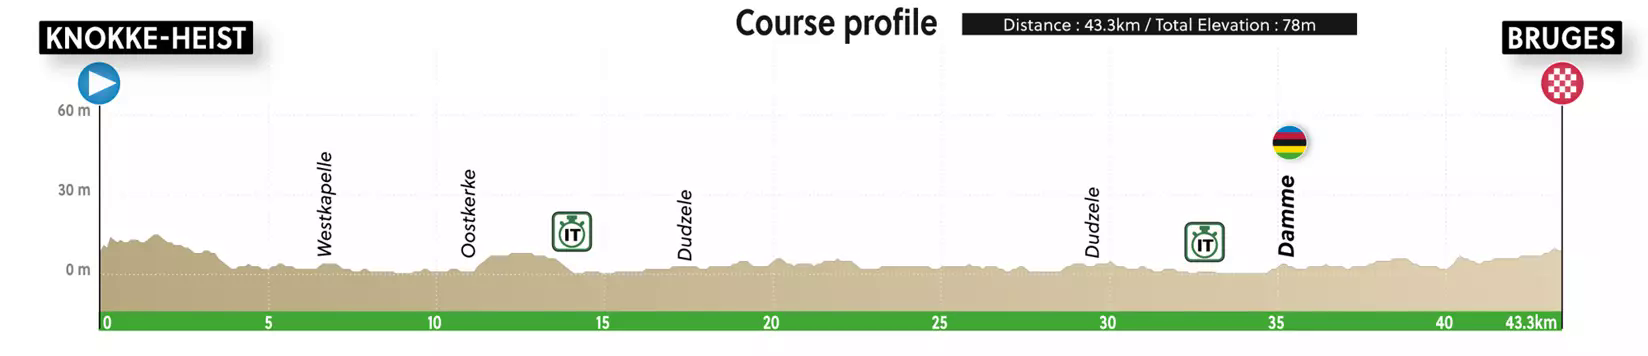
\includegraphics[width=1\columnwidth]{men-elite-individual-time-trial}
    \caption{course profile(from https://www.flanders2021.com)}
\end{figure}
We first find the course profile from https://www.flanders2021.com
then use the Reverse-Engineering Visualizations method developed by Jorge Poco1 and Jeffrey Heer in 2017\cite{poco2017reverse} to get the data we need about the racing track.
\section{Requirement 3}
\begin{enumerate}
    \item For each genre, the median of the various musical characteristics of all musicians for the entire genre is calculated as the musical characteristics
          for the entire genre, and we will still use the Pearson Correlation Coefficient we discussed in the last question. We will compare different similarity between two
          genres, and find the highest similarity $a$ that is allowed between genres songs will be classified to a certain genre if there is a higher similarity than $a$, and a song
          that can't be classified into all the genres we have known will be classified into a new genre. For all genres, their changes in musical characteristics will be show in
          a curve.

    \item One of the reason why genres are hard to distinguish is that most musicians were often influences by a group of other musicians from different genres, so there are
          come connections between nearly every two genres. Yet when what we want to find is not something that blurry, we want to know the relationship between the genres,
          so we set a standard below which the influence are ignored. It is clear that logically, if we want to draw a graph that show the causal relationship between the genres
          the graph show be an acyclic graph, thus the standard value should be the smallest value it can take to make the value an acyclic graph. The number, as we find out later
          by a few simple tests, is 45.
\end{enumerate}

\section{Requirement4}\Large
Whether there is an effect can be determined by directly calculating the mean (median) of the similarity between a pair  of notes and whether it is generally,
on average, higher than normal. Thus, we will iterate over each edge and, for each edge, find the similarity between the two nodes before and after, and for every
edge the calculation will give us a characteristic that has the highest similarity between the two note, those with a higher chance to be our "champion" will be considered
more contagious.
\section{Requirement 5}
To find the characteristics that might signify revolutions (major leaps) in musical evolution, we need to analyze those musicians that became active in the beginning of
a genre, they are exactly artists who represented revolutionaries (influencers of major
change) find the characteristics that are most different from the genre that the emerged from, they are most likely those we were seeking.
\newpage
\section{Requirement 6}
\begin{center}
    \huge \textbf{Rider's Guidance}
\end{center}\large
You have been training and focussing on this race for a while; you  have just progressed from youth races to your first junior race; you are experienced in riding. 
However, taking part in the race on the open road in a bunch is an exciting challenge, and you don’t want to make any mistakes. 
Understanding the techniques, skills, etiquette and rules will help keep the race safe and enjoyable for everyone. Now I must ask all of you to pay close attention to the instructions in the guide and use your power meter
to help you control your pace to meet its required so that you can make the best of yourself without hurting yourself with the high tensity of the race and your eager for
the champion. This knowledge can also significantly improve your chances of finishing in the best possible place in the results! 

Recently a new model has been developed to find the best racing strategy for each rider, from your trainings and races in the past, it was able to quantificat your ability
like stamina, recovery, critical power and maximum power the model will show you when to slow down and when to speed up, with a proper pace you will be able to ride 
fast and easy. 

A pre-performance routine means your attention stays in the present and only on elements that are task-relevant. It helps reduce anxiety, gets you to your optimal level 
of nerves, and improves concentration, focus and performance.

The routine gets you ready to compete, feeling comfortable you have done everything possible to reach the start line with the best preparation. The more you repeat and 
practise the routine, the more beneficial it is. I hope you have all remembered the instructions above, and it is ok if you didn't, you will remember them in a few routines.
Now go!
%%%%%%%%%%%%%%%%%%%%%%%%%%%%%%
\bibliographystyle{plain}
\bibliography{2022_MCM_ICM_Report}
\end{document}
\end
